% Very simple template for lab reports. Most common packages are already included.
\documentclass[a4paper, 11pt]{article}
\usepackage[utf8]{inputenc} % Change according your file encoding
\usepackage{graphicx}
\usepackage{url}
\usepackage{caption}
\usepackage{subcaption}

\title{\textbf{Distributed Artificial Intelligence and Intelligent Agents Homework 1}}
\author{KTH Royal Institute of Technology \\ 
		School of Information and Communication Technology \\
		Student:Fanti Machmount Al Samisti (fmas@kth.se) \\
		Student:August Bonds (bonds@kth.se)}

\begin{document}
	
\maketitle

\section{Introduction}

The purpose of this lab was to learn mobility in the Java Agent DEvelopment framework, the concept of cloning and moving agents between containers.

We also had to implement a multi-agent solution to the N-Queens problem.

This report serves primarily as an explanation of our solution, and some reasoning behind. Attached is all source code with descriptional comments.

\section{Task 1 - The N-Queens Problem}
The task was to implement a solution to the N-Queens problem using agents. This problem is normally solved with either a BFS or DFS over potential placement configurations. Since we did not want to rely on a centralized knowledge-repository (a stack or queue of configurations to try) we had to think differently.

Our implementation found solutions traversing the solution space in a DFS-like manner, but instead of operating on a shared datastructure, each agent would pass the current positioning of all predecessors plus its own position forward, and keep track of every tried position for itself given that predecessor configuration.

The agents thus communicated using only two kinds of messages. A "Go" message containing current positions sent to the successor, and a "Backtrack" message for telling a predecessor that the current branch is impossible.

When agent N found a possible placement given the N-1 predecessor positions, it would print the configuration and send a backtrack message for the algorithm to continue to find other configurations.
\section{Task 2 - Hands-on with Agent Mobility}

The task was to run at least two auctions, each one running in a different container, but with both artist manager agents and curator agents actually sending clones to do the auctioning/bidding and afterwards collecting the results in the original agent.

Our non-clone solution was using the ContractNetInitiator/Responder behaviors for auctioning, and this could neatly be expanded to cover clones.

To handle different behaviors of clones vs. originals we simply added/removed behaviors dependent on the name of the agent. We kept a copy of the source agent name for comparison, and let the clone agents add behaviors if they didn't have that name.

Any work done by clones was stored as static variables.

We then kept a counter for "returned agents", so that when all agents had returned we could execute an operation on the sum of the clones' work. An overview of this logic can be found in \ref{fig:results1}.
\begin{figure}
	\begin{center}
		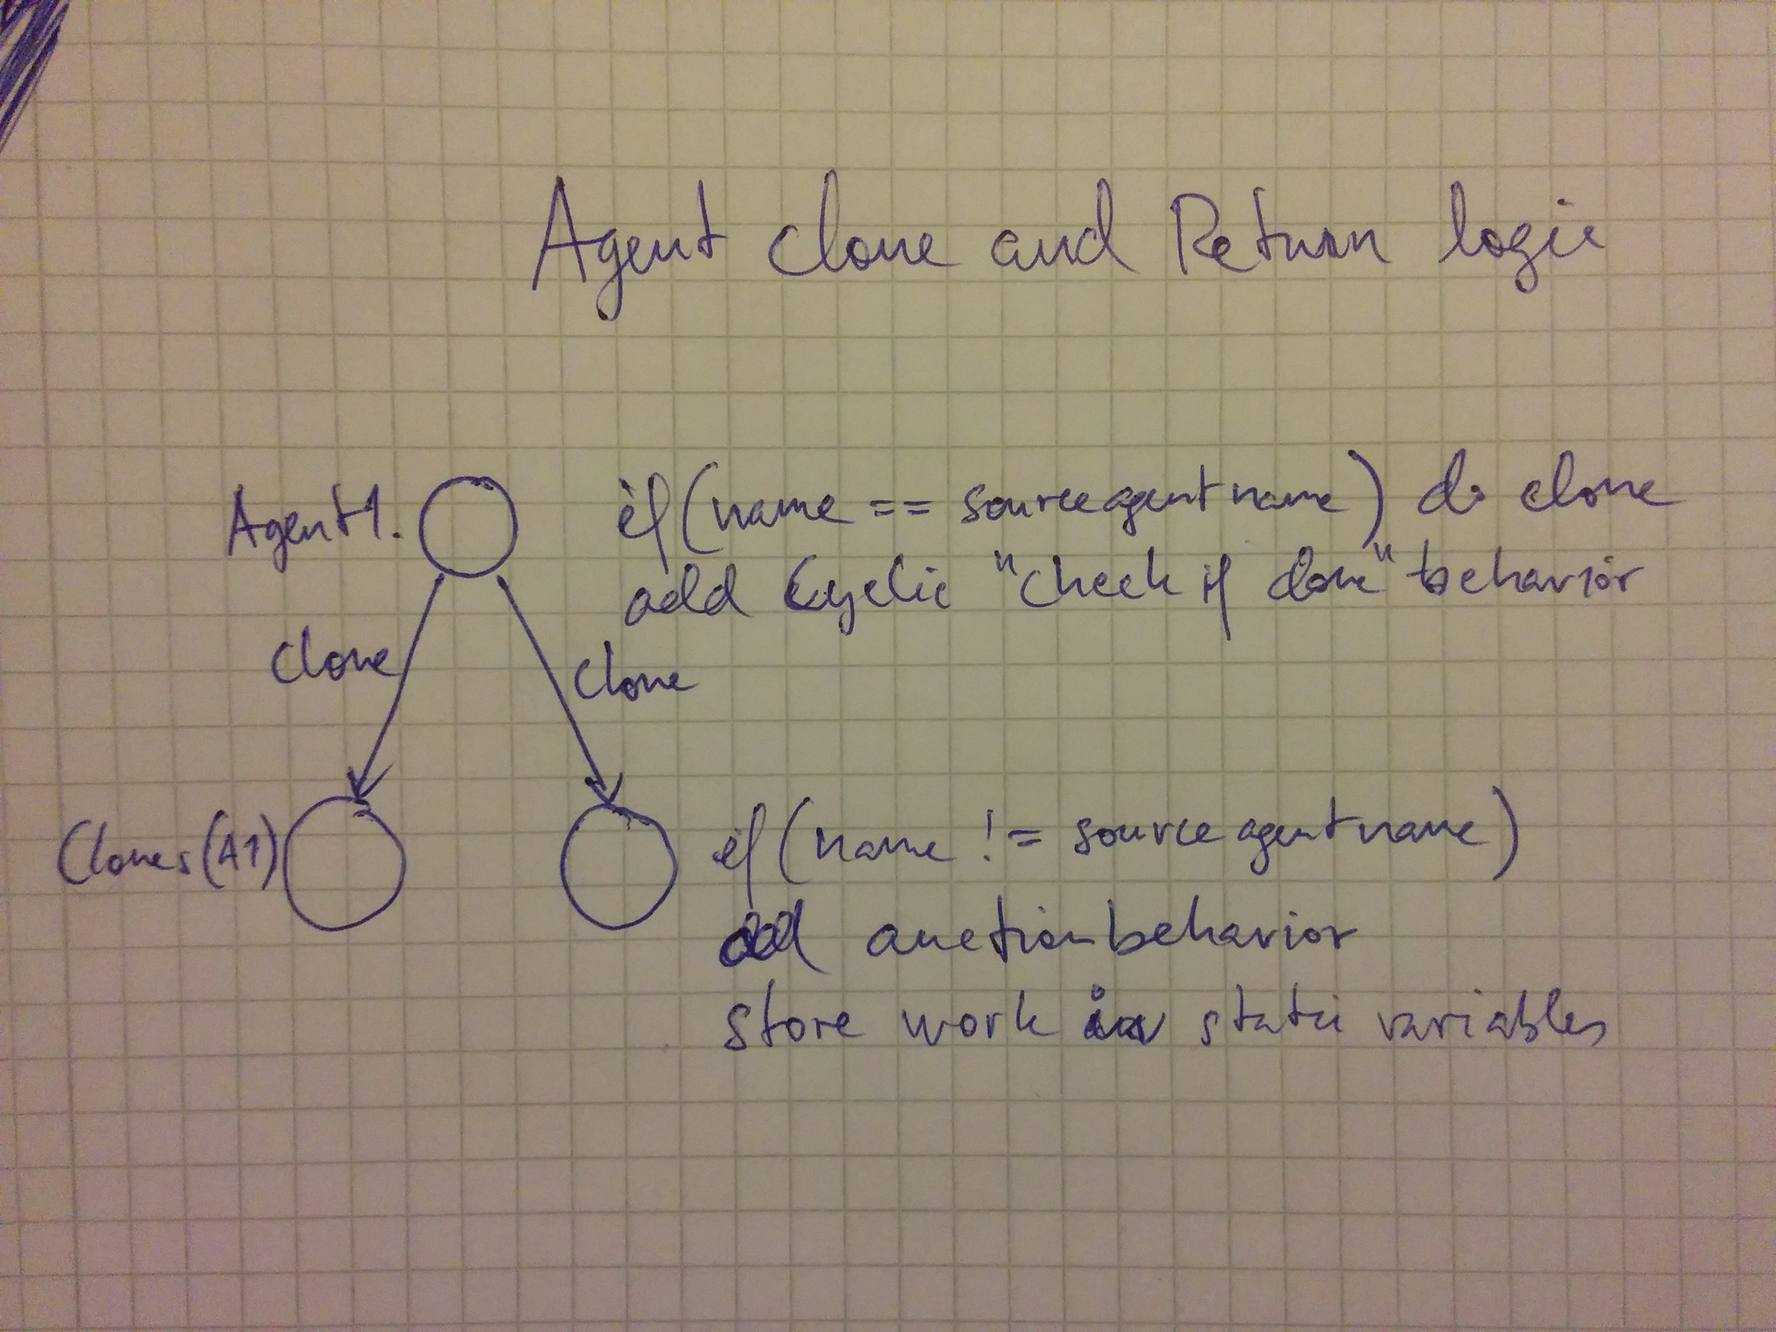
\includegraphics[width=\textwidth]{agentclonelogic.jpg}
		\caption{Overview of agent and clone logic }
		\label{fig:results1}
	\end{center}
\end{figure}

Timing when dealing with the creating and cloning of multiple agents turned out to be important. We had to add a delay before running any auctioneer code to make sure that all the curator clones were properly set up. 

\section{Running the code}
Import the project into IntelliJ as a Maven project and run Main.java with one argument for board size for N-Queens.

Import the project and run MainClone.java for task 2. 
\section{Evaluation}
In this lab we implemented a distributed solution to an algorithmic problem which we would normally be solving with non-distributed means. Additionally, by extending the previous homeworks we learned about agent mobility and cloning between containers.
\end{document}
